\chapter{DESENVOLVIMENTO DA SOLUÇÃO WEB}
\label{cap:web}
\setlength{\emergencystretch}{3em}

A parte web da solução é formada por dois projetos ASP.NET Core sobre o .NET 10 \cite{microsoft2026aspnet}: o \texttt{Pim.Web}, aplicação \textit{Model-View-Controller} (MVC) usada no escritório, e o \texttt{Pim.Api}, uma \textit{Minimal API} consumida pelo aplicativo. Ambos dependem da biblioteca \texttt{Pim.Core}, que concentra entidades, serviços de regra de negócio e acesso a dados (Capítulo~\ref{cap:arquitetura}). Este capítulo mostra como os conteúdos de Desenvolvimento Web com .NET foram aplicados em cada parte.

\section{Arquitetura da aplicação: HTTP e o \textit{pipeline}}

Toda interação da solução é uma transação HTTP: o cliente envia uma requisição com método, caminho, cabeçalhos e, quando necessário, um corpo, e o servidor devolve um código de status, cabeçalhos e a representação do recurso \cite{ietf2022http}. O protocolo é sem estado, isto é, cada requisição precisa trazer tudo o que o servidor necessita para atendê-la. Por isso o navegador envia um \textit{cookie} e o aplicativo envia um \textit{token} em todas as requisições (Seção~\ref{sec:autenticacao}).
No ASP.NET Core, o servidor Kestrel recebe a conexão e cria um \texttt{HttpContext}, objeto que reúne a requisição, a resposta, o usuário autenticado e os serviços disponíveis para aquele atendimento. O arquivo de inicialização de cada projeto (Program.cs) tem duas fases: primeiro registra os serviços no contêiner de injeção de dependência (\texttt{DbContext}, serviços do núcleo e autenticação); depois, já com a aplicação construída, monta o \textit{pipeline}, a sequência de \textit{middlewares} que trata cada requisição. Cada \textit{middleware} decide se chama o próximo e pode agir na ida e na volta, por isso a ordem de registro é decisiva \cite{araujo2018}. A Tabela~\ref{tab:pipeline} mostra o \textit{pipeline} do \texttt{Pim.Web}.

\begin{table}[htbp]
\centering
\caption{\textit{Pipeline} de requisições do Pim.Web, na ordem de execução}
\label{tab:pipeline}
\footnotesize
\begin{tabular}{|c|p{4.4cm}|p{9.2cm}|}
\hline
\textbf{\#} & \textbf{Componente} & \textbf{Função na solução} \\ \hline
1 & \texttt{UseExceptionHandler} & Fora do ambiente de desenvolvimento, captura falhas não tratadas e mostra uma página genérica, sem expor detalhes internos \\ \hline
2 & \texttt{UseHsts} e \texttt{UseHttpsRedirection} & Redirecionam HTTP para HTTPS e instruem o navegador a usar só conexões seguras \\ \hline
3 & \texttt{UseRouting} & Compara método e caminho com as rotas registradas e seleciona o \textit{endpoint} \\ \hline
4 & \texttt{UseAuthentication} & Lê o \textit{cookie} e preenche \texttt{HttpContext.User} com as \textit{claims} do usuário \\ \hline
5 & \texttt{UseAuthorization} & Confere se o perfil atende ao exigido pelo \textit{endpoint}; se não, interrompe e redireciona \\ \hline
6 & \texttt{MapStaticAssets} e \texttt{MapControllerRoute} & Servem CSS e JavaScript sem passar pelo MVC e executam a \textit{action} do \textit{controller} \\ \hline
\end{tabular}
\fonte{Elaborado pelo autor (2026)}
\end{table}

Na API, um \textit{middleware} próprio (\texttt{app.Use}) trata uma preocupação transversal: ele envolve a chamada ao próximo componente (\texttt{await proximo()}) em um bloco \texttt{try}, e, se algum serviço lançar \texttt{RegraNegocioException}, captura o erro na volta do \textit{pipeline} e responde \texttt{400} com a mensagem da regra, como ``RN10: esta caixa pertence a outro carregamento''.


\section{Roteamento, \textit{binding} e escolha do estilo}

O \texttt{Pim.Web} usa a rota convencional \texttt{\{controller=Home\}/\allowbreak\{action=Index\}/\allowbreak\{id?\}}: o endereço \texttt{/Carregamentos/\allowbreak Detalhes/7} executa o método \texttt{Detalhes(7)} do \texttt{Carregamentos\allowbreak Controller}. Na API, cada rota é declarada com \texttt{MapGet} ou \texttt{MapPost} e usa restrições de tipo, como \texttt{/recebimentos/\{id:int\}}; um identificador não numérico nem chega ao código e recebe \texttt{404}. Em seguida, o \textit{model binding} converte os dados textuais da requisição nos parâmetros do método, conforme a origem de cada um: o identificador vem da rota (\texttt{int id} em \texttt{/recebimentos/3/caixas}); o QR Code, da \textit{query string} (\texttt{string qr}); a chave da nota, do corpo JSON (\texttt{IniciarEntradaRequest}); os pedidos escolhidos, dos campos do formulário HTML (\texttt{List<int> pedidoIds}); os serviços, do contêiner de injeção de dependência (\texttt{EntradaService}); e o usuário, das \textit{claims} do \textit{token} ou do \textit{cookie} (\texttt{ClaimsPrincipal}).

A disciplina apresentou três estilos de aplicação no ASP.NET Core, e a escolha considerou o tipo de cliente e o tamanho de cada parte. O MVC, com classes \textit{controller}, \textit{views} Razor, filtros e convenções, foi adotado no \texttt{Pim.Web}, que tem oito áreas com listas, formulários e validação. A \textit{Minimal API}, com rotas declaradas como funções e pouca estrutura, foi adotada no \texttt{Pim.Api}, que tem poucas rotas e responde só JSON. O Blazor Server não foi adotado: ele mantém o estado de cada usuário no servidor por uma conexão SignalR permanente, recurso útil para telas muito interativas, enquanto aqui cada página MVC é uma requisição independente, sem conexão a manter.

\section{Aplicação web com MVC e Razor}

O \texttt{Pim.Web} tem um \textit{controller} por área (Pedidos, Carregamentos, Recebimentos, Veículos, Motoristas, Caixas, Conta e Início). Cada operação tem uma \textit{action} GET, que mostra o formulário, e uma POST, que o processa. Após uma gravação bem-sucedida, a \textit{action} redireciona para outra página e passa a mensagem de confirmação por \texttt{TempData}, padrão conhecido como \textit{Post/Redirect/Get}, que impede o reenvio do formulário ao atualizar a página. Quando um serviço recusa a operação por regra de negócio, o \textit{controller} captura a exceção e reapresenta o formulário com o motivo.

As \textit{views} usam um \textit{layout} único (\_Layout.cshtml), com o menu e o espaço do conteúdo, aplicado a todas as páginas por um arquivo de configuração das \textit{views} (\_ViewStart.cshtml). Trechos repetidos foram extraídos em \textit{partial views}: a de status (\_Status.cshtml) desenha a etiqueta colorida e é reutilizada em oito telas, e a de formulário (\_Formulario.cshtml) é o mesmo formulário nas telas de cadastro e de edição de motoristas. Os \textit{Tag Helpers} geram o HTML a partir do C\#: \texttt{asp-controller} e \texttt{asp-action} montam os endereços a partir das rotas, \texttt{asp-for} liga cada campo a uma propriedade do modelo e \texttt{asp-validation-for} exibe a mensagem de erro do campo.

A validação usa \textit{Data Annotations} nas entidades, como mostra o código a seguir. As mesmas regras são verificadas no navegador, pelo \textit{script} de validação incluído na página, e no servidor, pelo \texttt{ModelState}, que é a verificação que vale. Regras que dependem do banco, como placa repetida, são acrescentadas pelo \textit{controller} com \texttt{AddModelError}.

\begin{codeblock}[Validação por \textit{Data Annotations} e \texttt{ModelState} (Veiculo.cs e VeiculosController.cs)]{[Sharp]C}
[Required(ErrorMessage = "Informe a placa.")]
[StringLength(7, MinimumLength = 7, ErrorMessage = "A placa tem 7 caracteres...")]
public string Placa { get; set; } = "";
[Range(1, 1000, ErrorMessage = "O limite deve ser entre 1 e 1000 caixas.")]
public int LimiteCaixas { get; set; }                          // RN09
// no controller, ao cadastrar
if (await _db.Veiculos.AnyAsync(v => v.Placa == veiculo.Placa))
    ModelState.AddModelError(nameof(Veiculo.Placa), "Já existe ...");
if (!ModelState.IsValid) return View(veiculo);    // volta com as mensagens
\end{codeblock}

Dois filtros globais, registrados no \texttt{AddControllers\allowbreak WithViews}, valem para todas as \textit{actions}: o \texttt{AuthorizeFilter}, que exige login em qualquer página (apenas a tela de login é liberada com \texttt{[AllowAnonymous]}), e o \texttt{AutoValidate\allowbreak Antiforgery\allowbreak TokenAttribute}, que protege todos os formulários contra CSRF (Seção~\ref{sec:seguranca}). A interface usa o Bootstrap 5, com \textit{layout} responsivo. A Figura~\ref{fig:web} mostra a lista de carregamentos, com o progresso de bipagem atualizado pelo aplicativo, e a Figura~\ref{fig:webcriar}, a criação de um carregamento, que só oferece pedidos abertos.

\begin{sidewaysfigure}
\centering
\caption{Tela web: lista de carregamentos, com o progresso da bipagem}
\label{fig:web}
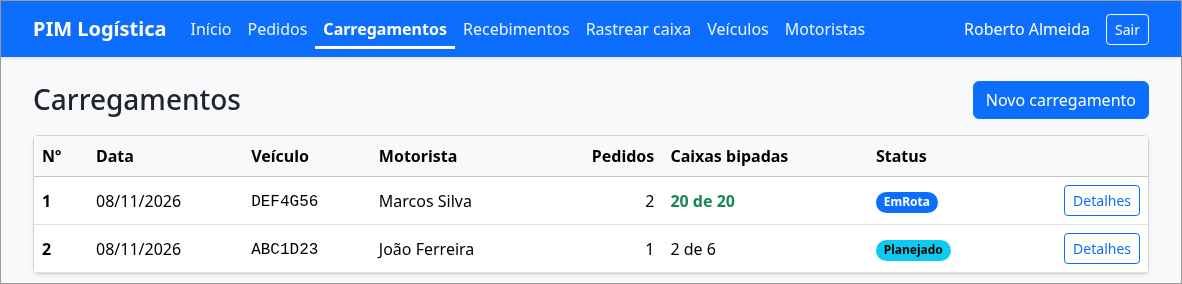
\includegraphics[width=23cm]{figuras/web_carregamentos.png}
\fonte{Elaborado pelo autor (2026)}
\end{sidewaysfigure}

\begin{sidewaysfigure}
\centering
\caption{Tela web: criação de um carregamento, que só oferece pedidos abertos}
\label{fig:webcriar}
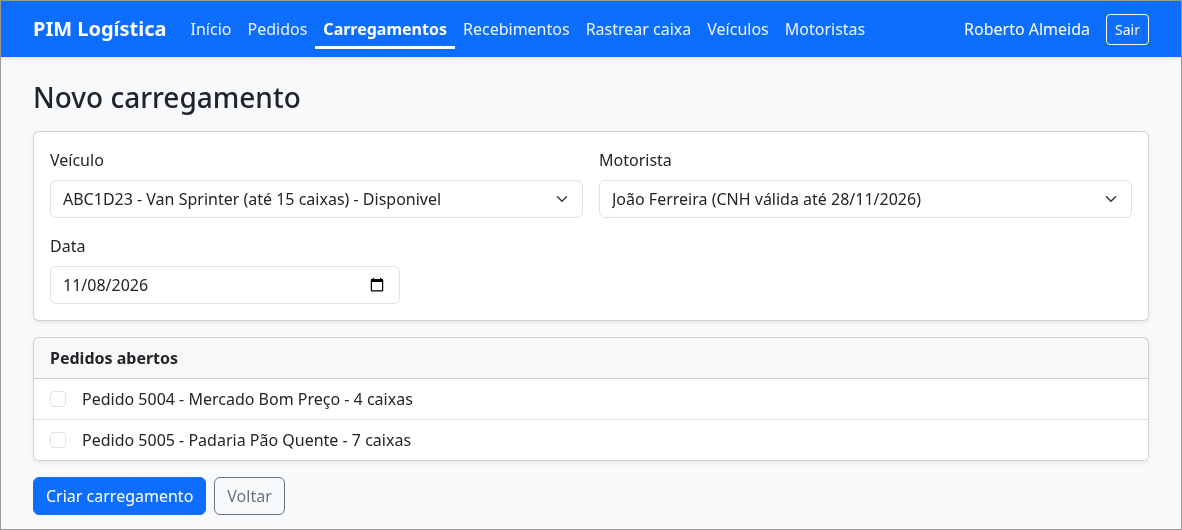
\includegraphics[width=23cm]{figuras/web_criar.png}
\fonte{Elaborado pelo autor (2026)}
\end{sidewaysfigure}

\section{Persistência com Entity Framework Core}

O acesso a dados usa o Entity Framework Core, mapeador objeto-relacional da plataforma. O \texttt{PimDbContext} expõe uma coleção (\texttt{DbSet}) por entidade e completa o mapeamento por convenção com configurações no método \texttt{OnModelCreating}, como os índices únicos e a proibição de exclusão em cascata. Ele é registrado com \texttt{AddDbContext}, que cria uma instância por requisição: tudo o que uma requisição altera é gravado em um único \texttt{SaveChangesAsync}, executado em uma transação.

O esquema é versionado por duas \textit{migrations}: \texttt{Inicial}, gerada a partir das classes, e \texttt{Triggers\allowbreak EProcedures}, que cria os objetos SQL do Capítulo 8. A classe \texttt{DadosIniciais} faz o \textit{seed} com a carga simulada do ERP. Em desenvolvimento, as \textit{migrations} são aplicadas na inicialização, por conveniência; em produção, essa aplicação passa a ser uma etapa própria da esteira de implantação (Capítulo 9). As consultas são escritas em LINQ e traduzidas para SQL parametrizado; as telas usam \texttt{Include} e \texttt{ThenInclude} para trazer de uma vez os dados relacionados, evitando uma consulta extra para cada linha exibida.

Nas aulas práticas, o padrão Repositório foi aplicado com uma interface própria e duas implementações, em memória e com o EF Core, trocadas em uma linha do registro de serviços. Nesta solução, o próprio \texttt{DbContext} cumpre os papéis de repositório e de unidade de trabalho \cite{fowler2006}, pois só há uma forma de armazenamento. A concorrência otimista com \texttt{RowVersion}, para a edição simultânea de um mesmo registro, fica como evolução.

\section{APIs REST}

A API segue o estilo REST \cite{fielding2000}: cliente e servidor separados, comunicação sem estado e interface uniforme, em que cada recurso tem um endereço, nomeado por substantivo no plural (\texttt{/recebimentos}), e o verbo HTTP indica a operação. Operações que não são simples criação ou alteração, como finalizar uma conferência, viraram sub-recursos de ação acessados por POST (\texttt{/recebimentos/\{id\}/finalizar}). As rotas são agrupadas por função e cada grupo exige um perfil, como mostra a Tabela~\ref{tab:rotas}.

\begin{table}[htbp]
\centering
\caption{Rotas da API consumidas pelo aplicativo}
\label{tab:rotas}
\footnotesize
\begin{tabular}{|p{6.6cm}|p{2.1cm}|p{3.6cm}|p{1.7cm}|}
\hline
\textbf{Método e rota} & \textbf{Perfil} & \textbf{Função} & \textbf{RF} \\ \hline
\texttt{POST /auth/login} & -- & Gera o token JWT & RF01 \\ \hline
\texttt{POST /portaria/} \newline \texttt{chegada-fornecedor} & Porteiro & Chegada de fornecedor & RF05 \\ \hline
\texttt{POST /recebimentos} \newline \texttt{GET /recebimentos/\{id\}} & Conferente & Inicia e consulta a entrada & RF06, RF07 \\ \hline
\texttt{POST /recebimentos/\{id\}/caixas} & Conferente & Bipa caixa e gera etiqueta & RF06 \\ \hline
\texttt{POST /recebimentos/\{id\}/} \newline \texttt{finalizar} & Conferente & Finaliza a conferência & RF07 \\ \hline
\texttt{GET /carregamentos/veiculo?qr=} & Operador & Carregamento do veículo & RF11 \\ \hline
\texttt{POST /carregamentos/\{id\}/caixas} & Operador & Bipa caixa no veículo & RF11 \\ \hline
\texttt{POST /portaria/saida} \newline \texttt{POST /portaria/volta} & Porteiro & Saída e volta pelo QR & RF12, RF14 \\ \hline
\texttt{GET /entregas} \newline \texttt{POST /entregas/\{id\}} & Motorista & Lista e registra entregas & RF13, RF16 \\ \hline
\texttt{POST /retornos/caixas} & Conferente & Bipa caixa que voltou & RF15 \\ \hline
\end{tabular}
\fonte{Elaborado pelo autor (2026)}
\end{table}

Os códigos de status fazem parte do contrato, pois o aplicativo reage pelo código, e não pelo texto: \texttt{200} devolve o recurso atualizado; \texttt{201}, com o cabeçalho \texttt{Location}, indica a entrada recém-criada; \texttt{400} traz a regra violada, que o aplicativo mostra com vibração; \texttt{401} (sem \textit{token}, vencido ou adulterado) leva de volta ao login; \texttt{403} indica perfil sem acesso; e \texttt{404}, rota ou identificador inexistente.

Os dados de entrada e saída são \textit{Data Transfer Objects} (DTOs) declarados como \textit{records}, como \texttt{LoginRequest}, \texttt{IniciarEntradaRequest} e \texttt{CaixaCriadaResponse}. As entidades nunca são expostas: isso evita devolver campos internos, como o \textit{hash} da senha, e permite mudar o banco sem quebrar o aplicativo. Cada grupo de rotas fica em um arquivo próprio da pasta de rotas (Endpoints), como método de extensão, e o arquivo de inicialização (Program.cs) apenas chama \texttt{app.MapPortaria()} e os demais. O código a seguir mostra o grupo da portaria: o \texttt{MapGroup} aplica de uma vez o prefixo, a etiqueta da documentação e o perfil exigido, e a rota não contém regra de negócio, apenas chama o serviço.

\begin{codeblock}[Grupo de rotas da portaria (Pim.Api/Endpoints/PortariaEndpoints.cs)]{[Sharp]C}
var grupo = app.MapGroup("/portaria").WithTags("Portaria (porteiro)")
    .RequireAuthorization(p => p.RequireRole("Porteiro"));
// RF12 / RN11: so sai com todas as caixas bipadas
grupo.MapPost("/saida", async (QrVeiculoRequest dados,
        PortariaService portaria, ClaimsPrincipal user) =>
    Results.Ok(await portaria.SaidaAsync(dados.Qr, user.UsuarioId())));
\end{codeblock}

Para os erros, a RFC 9457 define o formato \textit{Problem Details}, com os campos \texttt{type}, \texttt{title}, \texttt{status} e \texttt{detail} \cite{ietf2023problem}. Como o único cliente é o próprio aplicativo, optou-se por um corpo mais simples, com o campo \texttt{erro}; a adoção do \texttt{AddProblemDetails}, mantendo a mensagem da regra em \texttt{detail}, é a evolução prevista caso a API seja aberta a outros sistemas. As coleções da API não são paginadas, pois já são limitadas pelo contexto, como as entregas de um carregamento; no Web, a lista de pedidos tem filtro por status e busca pela \textit{query string}.

A documentação é gerada a partir do código (\textit{code-first}) pelo \texttt{AddOpenApi}, no padrão OpenAPI, e publicada em \texttt{/openapi/v1.json}; o Swagger UI apresenta essa documentação como uma página interativa, agrupada pelas etiquetas de cada grupo. Um arquivo de requisições HTTP (Pim.Api.http) traz uma requisição pronta por requisito. O cliente do aplicativo foi escrito à mão em Dart, mas poderia ser gerado do documento OpenAPI pelo OpenAPI Generator.

\section{Autenticação e autorização}
\label{sec:autenticacao}

Autenticação é descobrir quem é o usuário; autorização é decidir o que ele pode fazer. Os dois projetos verificam a senha da mesma forma, comparando-a com o \textit{hash} BCrypt guardado no banco, e criam as mesmas três \textit{claims}: identificador, nome e perfil. O que muda é como essa identidade acompanha as requisições seguintes, como compara a Tabela~\ref{tab:auth}.

\begin{table}[htbp]
\centering
\caption{Autenticação por \textit{cookie} no Web e por JWT na API}
\label{tab:auth}
\footnotesize
\begin{tabular}{|p{3cm}|p{5.5cm}|p{5.5cm}|}
\hline
\textbf{Aspecto} & \textbf{Web (\textit{cookie})} & \textbf{API (JWT)} \\ \hline
Cliente & Navegador & Aplicativo Flutter \\ \hline
Onde está a identidade & \textit{Ticket} cifrado dentro do \textit{cookie} & \textit{Token} assinado com HMAC-SHA256 \\ \hline
Envio & Automático pelo navegador & Cabeçalho \texttt{Authorization: Bearer} \\ \hline
Validade & 8 horas & 12 horas, configurável \\ \hline
Sem login & Redireciona para \texttt{/Conta/Login} & Responde \texttt{401} \\ \hline
Perfil sem acesso & Redireciona para \texttt{/Conta/AcessoNegado} & Responde \texttt{403} \\ \hline
Principal risco & CSRF, pois o \textit{cookie} vai sozinho & Roubo do \textit{token} \\ \hline
\end{tabular}
\fonte{Elaborado pelo autor (2026)}
\end{table}

O JWT é composto por três partes separadas por ponto: cabeçalho, conteúdo (\textit{payload}) e assinatura \cite{ietf2015jwt}. As duas primeiras são apenas codificadas em Base64url, e qualquer pessoa pode lê-las; por isso o \textit{token} carrega só o identificador, o nome e o perfil, nunca dados sensíveis. A assinatura é calculada com uma chave secreta que só a API conhece. Se alguém trocar o perfil de ``Motorista'' para ``Porteiro'' no conteúdo, a assinatura deixa de conferir e a requisição recebe \texttt{401}. Na validação, a API confere a assinatura, o emissor e a data de expiração.

\begin{codeblock}[Emissão do \textit{token} JWT no login (Pim.Api/Endpoints/AuthEndpoints.cs)]{[Sharp]C}
var token = new JsonWebTokenHandler().CreateToken(new SecurityTokenDescriptor
{
    Subject = new ClaimsIdentity(new[] {
        new Claim(ClaimTypes.NameIdentifier, usuario.Id.ToString()),
        new Claim(ClaimTypes.Name, usuario.Nome),
        new Claim(ClaimTypes.Role, usuario.Perfil.ToString()) }),
    Issuer = config["Jwt:Emissor"],
    Expires = expira,                                   // agora + 12 horas
    SigningCredentials = new SigningCredentials(chave, SecurityAlgorithms.HmacSha256)
});
\end{codeblock}

A validade de 12 horas cobre um turno, e o \textit{logout} no aplicativo descarta o \textit{token}. Como o JWT não é consultado no servidor, um \textit{token} copiado vale até expirar; a evolução indicada é o par \textit{access token} curto e \textit{refresh token} revogável, com o \textit{token} guardado em armazenamento cifrado do aparelho.

\begin{table}[htbp]
\centering
\caption{Perfis de acesso e funções liberadas}
\label{tab:perfis}
\footnotesize
\begin{tabular}{|p{2.6cm}|c|p{10cm}|}
\hline
\textbf{Perfil} & \textbf{Canal} & \textbf{Funções} \\ \hline
Gerente & Web & Todas as telas web, cancelamento de pedidos, aprovação de entradas e rastreio de caixas \\ \hline
Programador & Web & Pedidos, carregamentos e consulta de veículos \\ \hline
Frota & Web & Cadastro de veículos e motoristas, manutenção e QR Code \\ \hline
Comercial & Web & Consulta de pedidos \\ \hline
Conferente & App & Entrada de caixas e retorno \\ \hline
Operador & App & Carregamento do veículo \\ \hline
Porteiro & App & Chegada de fornecedor, saída e volta de veículos \\ \hline
Motorista & App & Registro das entregas do seu carregamento \\ \hline
\end{tabular}
\fonte{Elaborado pelo autor (2026)}
\end{table}

A autorização é feita por papéis (\textit{roles}). No Web, cada \textit{controller} ou \textit{action} declara os perfis aceitos, por exemplo \texttt{[Authorize(Roles = "Gerente,Frota")]} no cadastro de veículos; na API, cada grupo usa \texttt{RequireRole}. O menu do \textit{layout} esconde os itens que o perfil não pode usar, mas isso é apenas interface: quem digita o endereço de uma página proibida é barrado pelo atributo e levado à tela de acesso negado. Há ainda autorização por recurso: o motorista só vê e registra as entregas do carregamento em que está escalado, pois o serviço compara o motorista do carregamento com o identificador lido do \textit{token}, e não com um valor enviado pelo aplicativo.

O ASP.NET Core Identity oferece cadastro de usuários, regras de senha, bloqueio após tentativas erradas e dois fatores. Ele não foi adotado porque os usuários são poucos, criados pela empresa e com perfil fixo; uma tabela \texttt{Usuarios} com BCrypt atende ao cenário. O bloqueio após tentativas erradas, que o Identity traria pronto, fica registrado como evolução. OAuth 2.0 e OpenID Connect não se aplicam, pois não há login com contas de terceiros. O CORS também não foi habilitado: ele só é exigido por navegadores em chamadas entre origens diferentes, e o único cliente da API é um aplicativo nativo.

\section{Segurança e configuração por ambiente}
\label{sec:seguranca}

Além da autenticação, foram aplicados: HTTPS com HSTS; \textit{token} antifalsificação em todos os formulários, para que outro site não envie um formulário em nome do usuário (CSRF); \textit{cookie} inacessível ao JavaScript (\texttt{HttpOnly}) e cifrado pelo \textit{Data Protection}; validação no servidor; SQL parametrizado pelo EF Core; e CPF mascarado nas telas.

A configuração é lida em camadas, e a última fonte prevalece: o arquivo de configuração geral (appsettings.json), o arquivo do ambiente (appsettings.\allowbreak\{Ambiente\}.json), segredos de usuário (apenas em desenvolvimento), variáveis de ambiente e linha de comando. O ambiente é definido pela variável \texttt{ASPNETCORE\_\allowbreak ENVIRONMENT};, e o \texttt{Pim.Web} só ativa a página de erro genérica fora de \texttt{Development}. Assim, a mesma imagem roda em qualquer ambiente, e a variável \texttt{Jwt\_\_Chave} substitui a chave \texttt{Jwt:Chave} do arquivo.

Hoje, a chave do JWT e a senha do banco de desenvolvimento estão no arquivo de configuração (appsettings.json), o que só é aceitável localmente; o correto é usar \textit{User Secrets} no desenvolvimento e variáveis de ambiente alimentadas pelo Azure Key Vault em produção (Capítulo 9). Em contêineres, as chaves do \textit{Data Protection}, que cifram o \textit{cookie}, devem ficar fora do contêiner e ser compartilhadas entre instâncias, senão cada reinício desconecta os usuários.

\section{Estrutura administrativa e integração entre módulos}

A estrutura administrativa é definida pelos perfis da Tabela~\ref{tab:perfis}, e cada canal aceita apenas os seus perfis no login. 
A integração ocorre em dois níveis. No código, Web e API usam os mesmos serviços do \texttt{Pim.Core}; assim, cada regra vale igualmente em qualquer canal. Nos dados, ambos usam o mesmo banco, e uma caixa bipada no celular aparece na hora no progresso exibido no Web.
